\documentclass[]{report}

\usepackage{graphicx}
\usepackage[letterpaper, portrait, margin=1in]{geometry}

\begin{document}

\begin{titlepage}
	\begin{center}

	\huge{\bfseries Determination of Mineral Oil Nuclei Properties Using Nuclear Magnetic Resonance}\\
	
	\bigskip
		
	\textit{\Large Abstract}\\
	
	\medskip
	
	\normalsize 
	
Various qualities of mineral oil nuclei are observed by the processes of nuclear resonance. A radio frequency is applied to a permanent magnet with a sample of mineral oil situated in the center. A resonance frequency for the nuclei is determined to be $15.42248^{+0.046}_{0.052} $ MHz. A free induction decay from a 90 degree pulse is observed and is used to determine the gradient field as $\Delta B_{0} = 3.63*10^{-7} \pm 1.65*10^{-8}$ tesla/rad. The spin lattice relaxation time $T_{1}$ is found to be $16.697 \pm 3.695 $ ms. The spin spin relaxation time $T_{2}$ is determined by the Hahn, Carr-Purchell, and Meiboom-Gill methods, with a value obtained as $18.4409 \pm 0.34106 $ ms from the Meiboom-Gill with the delay time set to 0.8 $\mu$ s, which we decided as yielding the most accurate value. These different methodologies are compared and an analysis for errors is included.
	
	\line(1,0){0} \\

	\textsc{\normalsize Andreas Kooi \\
	Ronaldo Rodriguez \\}
	\textsc{\Large March 1, 2019}\\
	[4cm]
	\end{center}
	
	\begin{flushright}
	\textsc{\large 
	Physics 134 Laboratory \\
	Arthur Ramirez, Ph.D. \\
	University of California, Santa Cruz \\}
	
	\end{flushright}
	
\end{titlepage}



\section{Introduction and Theory}


\subsection{Background}

Pulsed Nuclear Magnetic Resonance, P-NMR for short, is built on the foundation of aligning the magnetic moments of nuclei with a magnetic field, resulting in a readable signal decay back to equilibrium after a magnetic pulse is applied.
Two important aspects of NMR are the spin lattice relaxation time $T_{1}$ and spin-spin relaxation time $T_{2}$. Different materials have unique $T_{1}$ and $T_{2}$ decay times, making these two properties of materials important in practical applications such as Magnetic Resonance Imaging machines, which are used to medically diagnose medical conditions in living tissue.
Different methodologies behind the practice were developed around the 1950's. These include the two pulse spin echo method by Erwin Hahn and the multiple-pulse methods of and Carr Purcell and the Meiboom-Gill for determining $T_{2}$. 

\subsection{Optical aberrations as described by Zernike Polynomials}



\subsection{Magnetic alignment of samples and their properties}

Atomic nuclei– protons and neutrons, are fermion particles with quantized spins $\pm 1/2$, and thus have corresponding quantized magnetic moments. If a homogenous magnetic field is applied in an appointed +z direction, the magnetic energy U is given by 

\begin{equation}
$$$
U = - \mu_{z} * B_{0}
$$$
\end{equation}

where $\mu_{z}$ denotes the magnetic moment and B is the external magnetic field. The magnetic moment is $\mu = \gamma J$, where $\gamma$ is a nucleus-specific gyromagnetic ratio and J is the quantized angular momentum corresponding to $\pm \frac{1}{2} \hbar$, $\hbar$ being Planck's constant. For our sample of mineral oil, we take into account the resonance of hydrogen atoms, or, protons, solely into account, which has a $\gamma$ value of $2.675*10^{8} \frac{rad}{sec*tesla}$.
 
Therefore, when an external field value $B_{0}$ is zero in (Eq. 1), a zero magnetic energy state that consists of two degenerate states is expected. When the external field is nonzero, two quantized values of energies are expected– with an energy difference $\Delta U = h \omega_{0}$.

For a sample of large nuclei, the total alignment is dependent on how many of the nuclei are in the spin half state versus the spin negative half state(otherwise equal and opposite spins would cancel), and is described by a thermal Boltzmann equilibrium. At a time t, the instantaneous magnetization of a sample is given by (Eq. 2).

\begin{equation}
$$$
M_{z}(t) = ( N_{1}(t) - N_{2}(t) ) \mu
$$$
\end{equation}

which depends on the difference of the nuclei states,  $N_{1} - N_{2}$ and the magnetic moment $\mu$.
The equilibrium magnetization is given by (Eq. 3).

\begin{equation}
$$$
M_{0} = ( N_{1} + N_{2} ) \frac{\mu^{2} B}{kT}
$$$
\end{equation}

where  $N_{1} + N_{2}$ illustrates that all spins are aligned during equilibrium. k is the Boltzmann constant and T denotes thermal temperature.


\subsection{$T_{1}$: The Spin Lattice Relaxation Time}

When a sample is introduced to an external +z-direction B field, the instantaneous magnetization $M_{z}(t)$ approaches the thermal equilibrium magnetization $M_{0}$ exponentially, as pictured in (Fig. 1), and the time constant is $T_{1}$.

\begin{figure}[h]

\centering
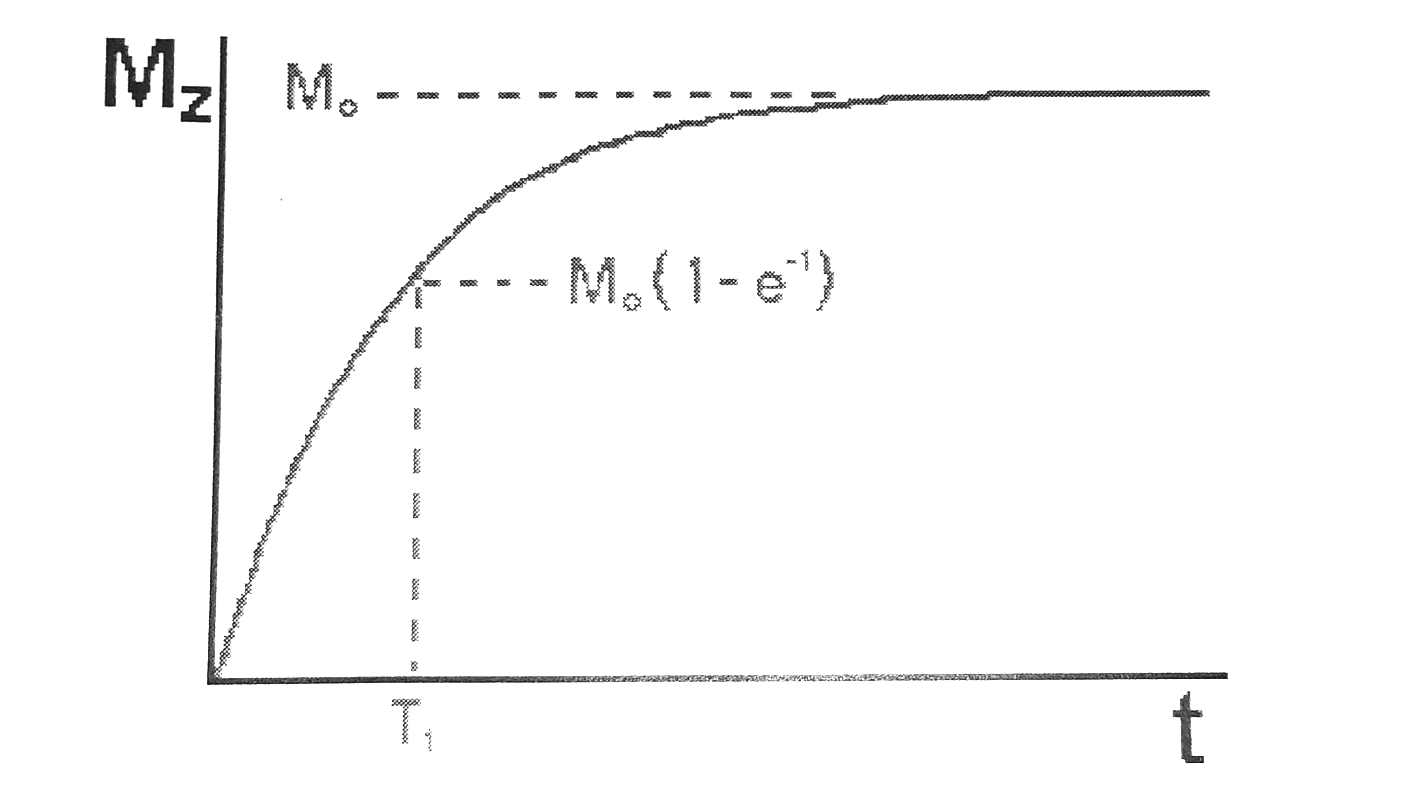
\includegraphics[width=6cm]{T1Decay} 

\caption{$T_{1}$ is the time it takes for the instantaneous magnetic alignment $M_{z}(t)$ to reach a value of $M_{0} (1 - e^{-1}$.}

\end{figure}

In order to find $T_{1}$ for the mineral oil sample, a 180-degree pulse is initiated so that the +z aligned magnetic nuclei in the sample can flip towards the -z direction, and they will accordingly realign to the magnetic field again with the described exponential. A 90 degree pulse is introduced shortly after the 180 degree pulse so that the relaxations can be read as an x-y decay. -z axis to +z axis decays and vise versa are not read off as signals. From a classical perspective, this is because a 180 degree torque is not read, and is more like a switch, but a perpendicular torque(on the x-y plane) is.

Setting the initial conditions for the differential rates to follow the 180 to 90 degree pulse method results in the following relationship between the voltage amplitude and time:

\begin{equation}
$$$
A(t) = A_{0} | 2e^{\frac{-t}{T_{1}}} - 1 | 
$$$
\end{equation}

\subsection{$T_{2}$: The Spin-Spin Relaxation Time}

$T_{2}$ is the time it takes for the nuclei spins to relax from an equilibrium x-y plane magnetization to the external +z magnetization. Under ideal circumstances where the magnetic field is perfectly homogenous, this is the FID, Free Induction Decay, constant. Each atom in the nuclei has a local magnetic field which interacts with neighboring nuclei. For this reason, different materials have unique $T_{2}$ values.
Magnetic field inhomogeneity results in the FID constant to be different than $T_{2}$ since spins in the stronger field areas will de-phase more quickly than average and spins in the weaker field areas will de-phase more slowly.
The resulting FID constant value will therefore be due to effects of $T_{1}$, $T_{2}$, and for the most part, from the field inhomogeneity. It is modeled as $T_{2}^{*}$:

\begin{equation}
$$$
\frac{1}{T_{2}^*} = \frac{1}{T_{2}} + \frac{1}{T_{1}} + \gamma \Delta B_{0} 
$$$
\end{equation}

To minimize these effects, a 180 degree pulse is applied after the 90 degree pulse, which will cause a convergence of the out of phase spins from the field inhomogeneity. When all spins converge and decay after the 180 degree pulse, a signal is produced, known as the echo signal. The echo has a smaller amplitude due to the local magnetic fields preventing every possible spin from relaxing. The difference in amplitude are due to the effects of the material's $T_{2}$ value. 
The Hahn method makes use of one such two pulse sequence and compares the echo amplitude to the initial amplitude.
The Car-Puchell method has numerous 180 degree pulses instead of one, and the echo amplitudes for each 180 degree pulse decays with the exponential $T_{2}$ constant. Because it is likely for the 90 degree and 180 degree pulses to not be exact, this method compounds the degree error for each 180 degree pulse iteration and the $T_{2}$ value is underestimated. The Meiboom-Gill method takes this into account by rotating the spins about the x axis in order to cancel compounding errors and is the most accurate. 

\section{Apparatus}

A permanent magnet manufactured by Teach-spin is used in conjunction with a Pulsed NMR Teachspin Spectrometer and an oscilloscope. The spectrometer consists of three modules: the synthesizer, the pulse programmer, and the receiver.
The pulse programmer serves to provide manual adjustments for the width of pulses, the delay time between the pulses, and the repetition time for the total pulse pattern. There are two types of pulses the programmer provides– an A and B pulse. There is one A pulse. After the adjusted delay time, a selectable amount of 0 to 99 B pulses takes place, each repeating themselves following the previous pulse after the delay time passes. The last B pulse indicates the end of the pulse sequence. The repetition time is the time between each sequence to repeat itself. Both the A and B pulses can be adjusted for their width.
The synthesizer is wired to the permanent magnet and is used to adjust the frequency applied to the permanent magnet.
The receiver module amplifies the signal received from the magnet and can be compared with the synthesizer input signal using the built-in mixer. It can also provide readings of the signal envelope, that is, the maximum positive amplitudes.
All of these components and their relations can be seen in (Fig. 3).

\begin{figure}[h]

\centering
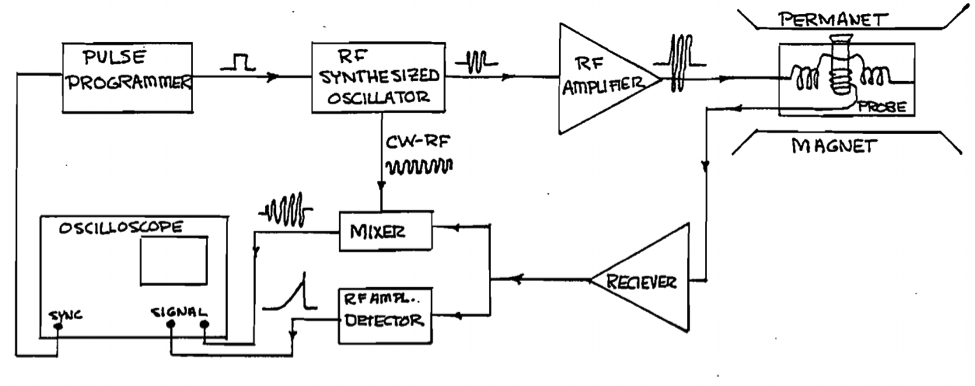
\includegraphics[width=9cm]{schematic} 

\caption{Schematic of the spectrometer}

\end{figure}


\section{Procedure}

\subsection{Determining the Resonance Frequency by Minimizing the Beat Frequency}

For all of the decay experiments, the programmed frequency needs to be at the same frequency where the hydrogen nuclei resonate with a maximum output. This occurs when the beat pattern of the mixer is minimized and neither the programmer signal or the received signal are interfering with each other. 
Adjusting the coarse adjust and fine adjust knobs led to a value of $15.42248^{+0.046}_{0.052} $ MHz, where the uncertainty marks the frequency displacement that results in an obvious non-resonant frequency.

\section{Results}

\subsection{Magnetic Field Gradient}

(Eq. 5) illustrates the observed FID decay constant, $T_{2}^*$, which is a result of the magnetic field inhomogeneity and $T_{2}$ and $T_{1}$. Since the majority of effects occur due to the inhomogeneity(which is why the two pulse method was designed to minimize it), $T_{2}$ and $T_{1}$ can be approximated to be large values, simplifying $T_{2}^*$ as an inhomogeneity approximation: 

\begin{equation}
$$$
\frac{1}{T_{2}^*} = \gamma \Delta B_{0} 
$$$
\end{equation}

To determine the observed FID constant $T_{2}^*$, an x-y plane pulse (90 degrees) was calibrated as $6.7 \pm 0.01$ $\mu s$ , which resulted in the largest signal response, and applied. Each pulse width, in ms, is determined using the cursor function on the oscilloscope. The time constant of the exponential decay was determined with a sample of six pairs of points as $10.3 \pm 0.466$ ms, where the uncertainty is determined from the standard deviation of all the individual time constant calculations. From this value, the magnetic field inhomogeneity is found as $\Delta B_{0} = 3.63*10^{-7} \pm 1.65*10^{-8}$ T. The attached uncertainty is due to the $T_{2}^*$ uncertainty, partially differentially propagated with respect to time from (Eq. 6).

\subsection{$T_{1}$}

Following the theory in section $0.1.3$, the A pulse is set up to be 180-degrees by doubling the width of the 90 degree pulse. Therefore, the A pulse is set to be $13.4 \pm 0.01$ $\mu s$. One B pulse is turned on, set to 90 degrees.
A range of data was collected for various times and is plotted as follows:

\begin{figure}[h]

\centering
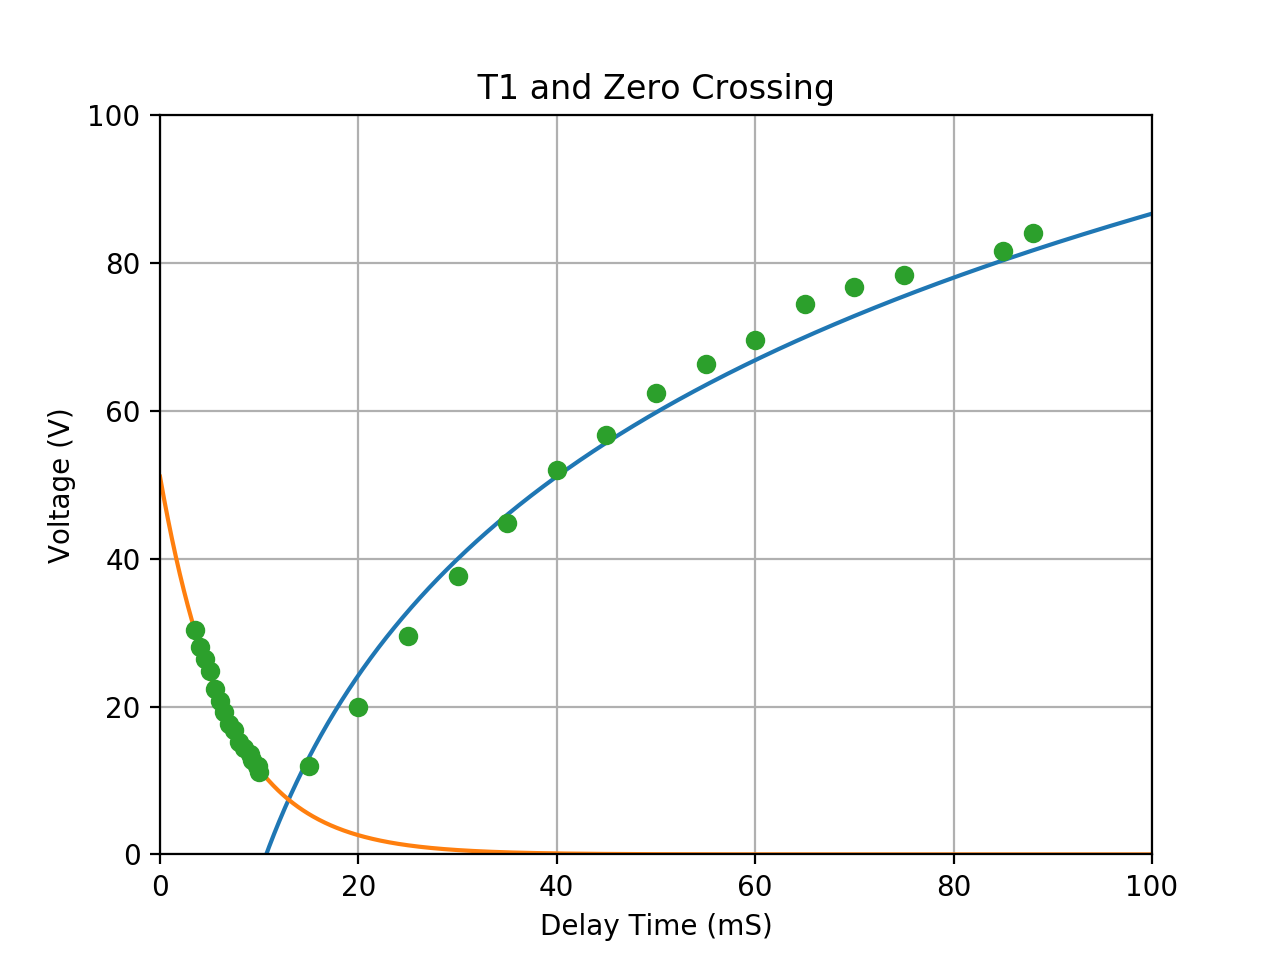
\includegraphics[width=8cm]{T1Plot} 

\caption{Decay from a 180 to 90 degree pulse. Green data points resemble data. The orange line fit is $y = -85.9 + 38.8ln(x)$. The blue line fit is $y = 51.1e^{-0.149x}$. The intersection of the two functions is the zero crossing time, determined to be $t_{0} = 11.573368 \mu s$. Due to systematic noise, the voltage at $t_{0}$ is vertically offset from zero, but should not have an impact on the time scale since it is a voltage displacement.}
\end{figure}

A value of $T_{1}$ is calculated by using the zero crossing method. This assumes that (Eq. 4)'s voltage amplitude is zero at a given time $t_{0}$. Rearranging the equation under this condition yields $T_{1} = \frac{t_{0}}{ln(2)}$. Using $t_{0}$ (see (Fig. 4)), $T_{1} = 16.697 \pm 3.695$ ms. The uncertainty for the value is determined by two factors: the voltage amplitude fluctuation and the uncertainty in the range of data values.
The voltage amplitude fluctuation was determined by seeing how much a particular voltage reading would deviate. The result was not much: a deviation of $0.641$ V. Next, this deviation was applied to the data(known as the bump up/down method) and the resulting fitting equations to see how it impacted $T_{1}$. The resulting range is small: $\pm 0.070115$ ms.
The majority of uncertainty occurs due to a lack of data recorded around the zero crossing, so an added on uncertainty is half the distance between the two closest points in the region, or, $\pm 3.5$ ms. 

\subsection{$T_{2}$}


\subsubsection{Hahn Two-Pulse Spin-Echo Method}

The A pulse was set to 90 degrees and the B pulse to 180 degrees. The uncertainty was found using a bump/up down method with respect to the observed amplitude fluctuations. The resulting decay is plotted in (Fig. 4) and results in $T_{2} = 13.28 \pm 0.68737$ ms.

\begin{figure}[h]

\centering
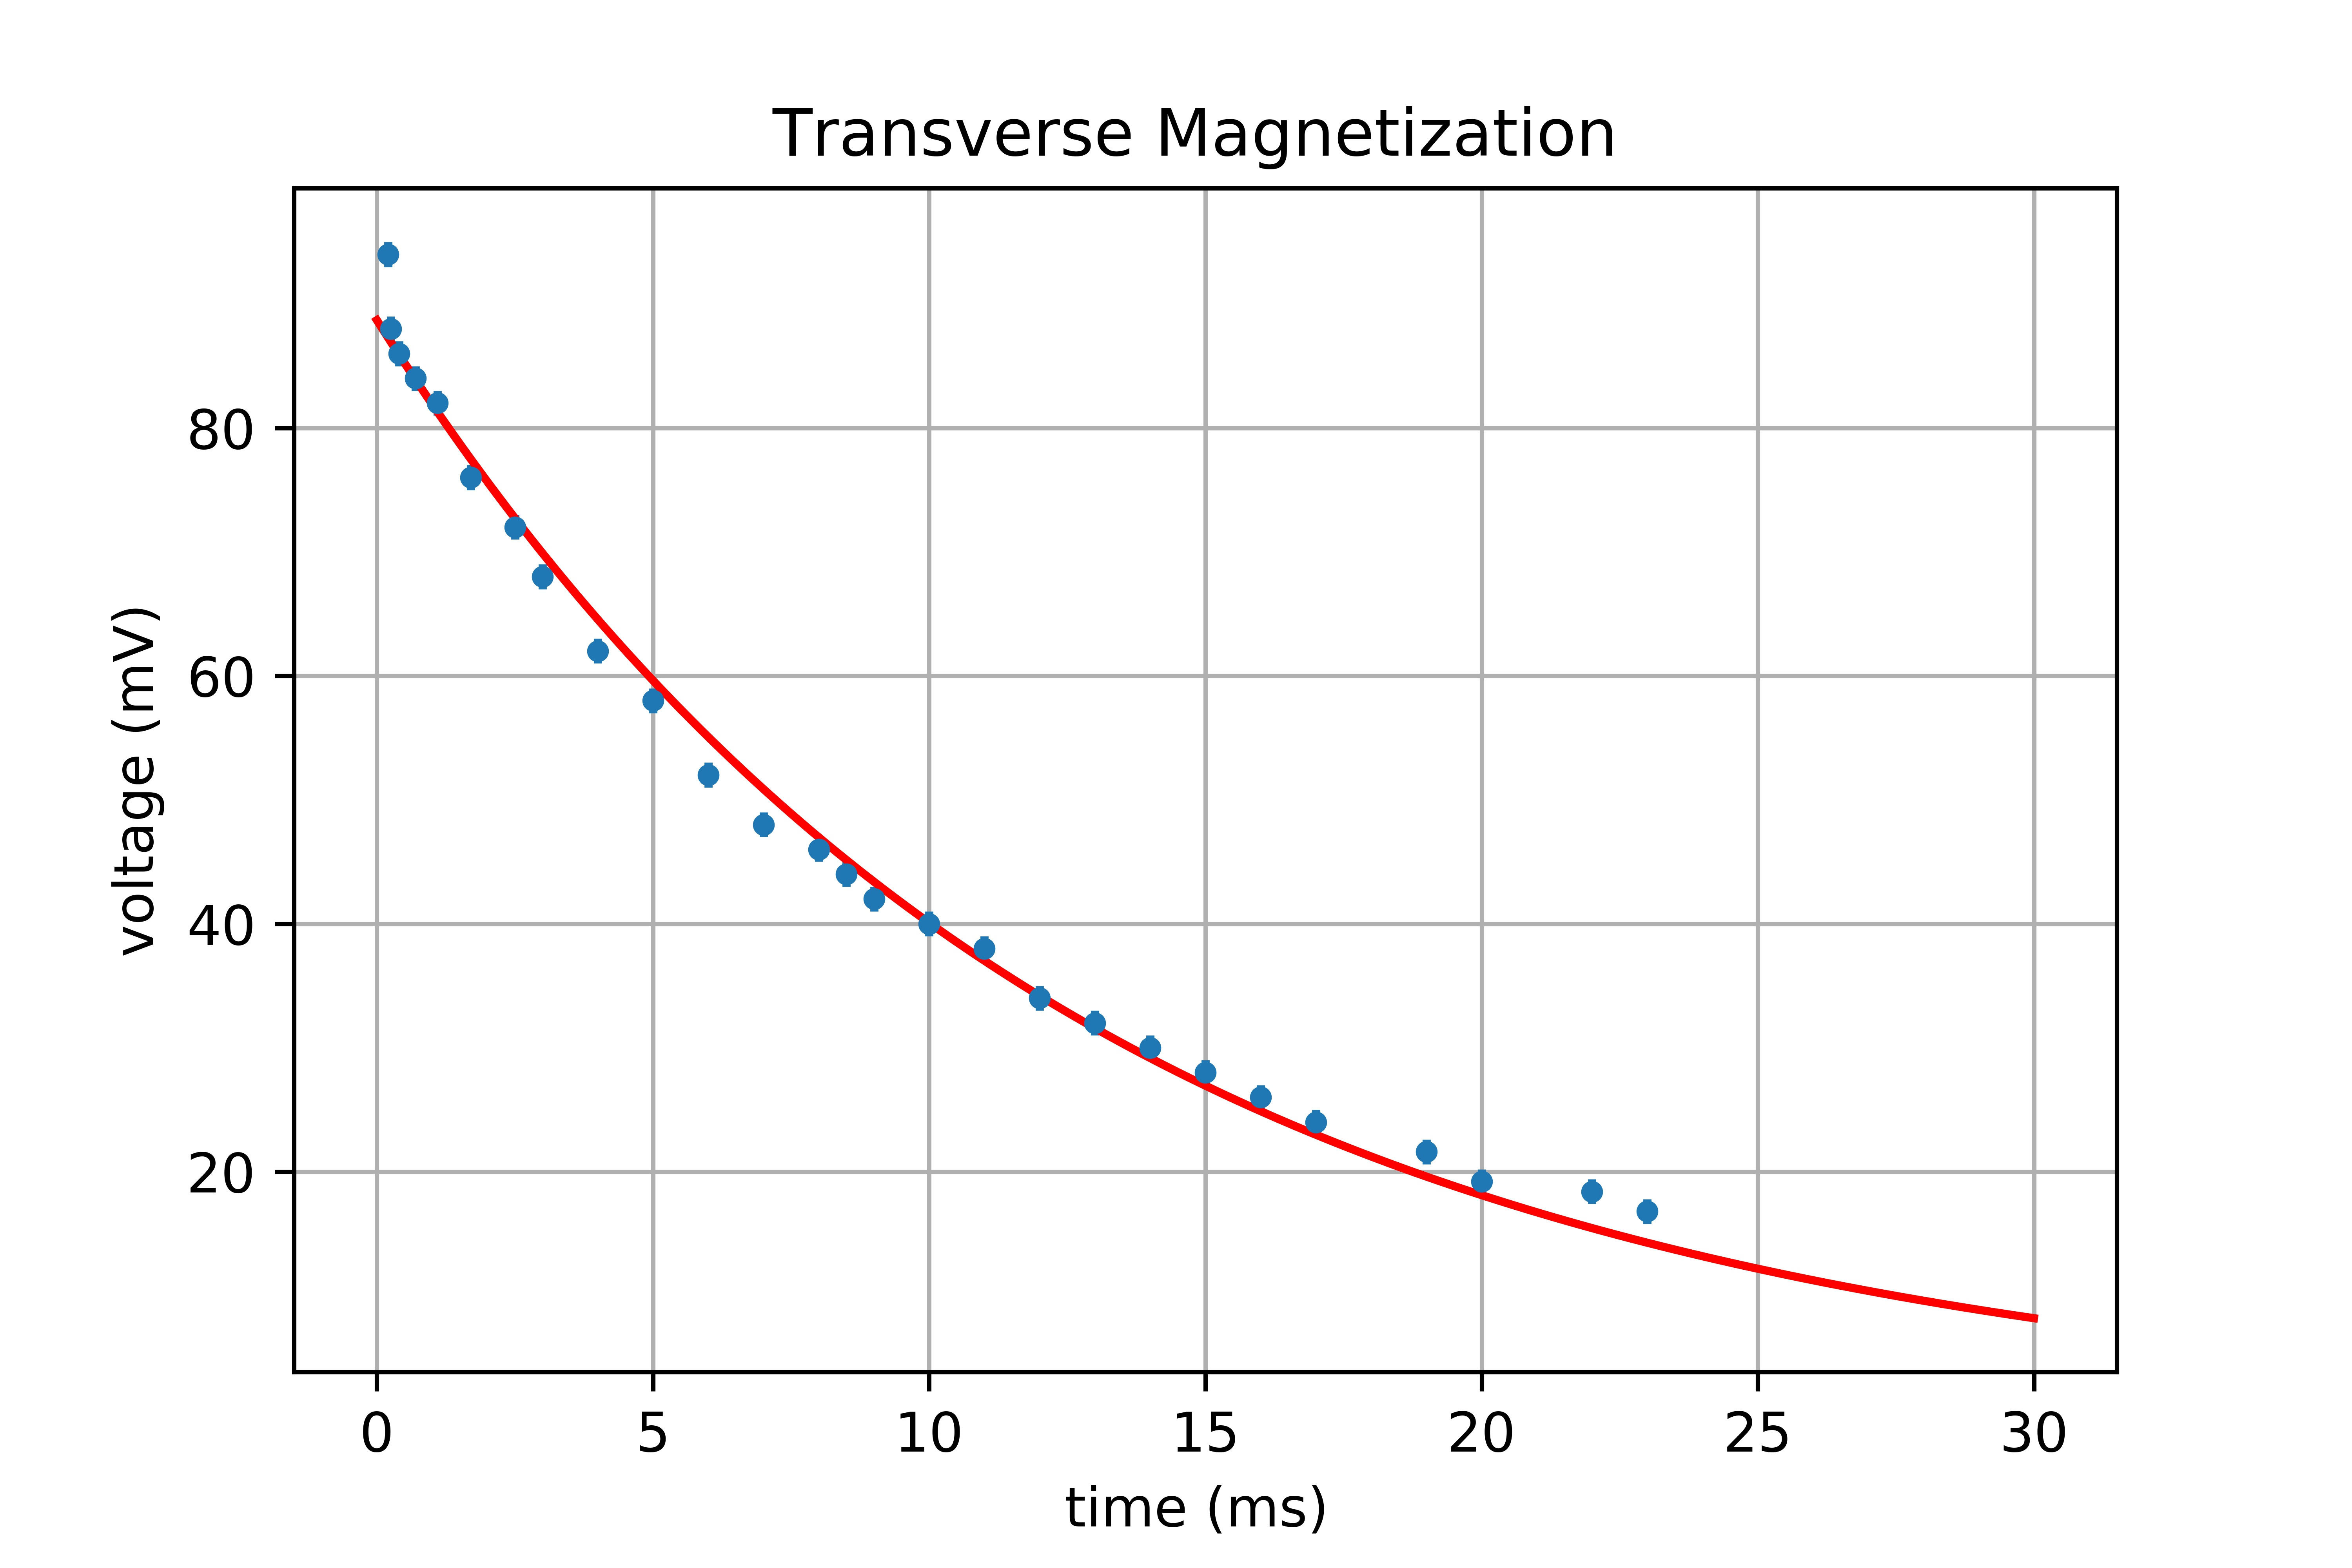
\includegraphics[width=10cm]{Hahn} 

\caption{The decay observed for the Hahn Two Pulse Method of finding $T_{2}$ along with the fitted exponential which yields $T_{2}$. Vertical error bars are 1.046 mV, determined by amplitude flucuations.}
\end{figure}

\subsubsection{Carr-Purcell Multiple Pulse Method}

Multiple Carr-Purchell and Meiboom-Gill runs were taken, each for the delay times set to 0.5, 0.6, 0.7, and 0.8 ms. The values of $T_{2}$ were plotted and tabulated for each of these, and are available upon request. The resulting values are lob-sidedly distributed: larger delay times had larger decay constants. This is because with a shorter delay time between the B pulses, there is less time for a full decay and therefore the exponential is condensed as shorter. For this reason, my partner and I concluded that the data for the delay set to 0.8 ms are the most accurate. The Carr-Purchell method resulted in a quicker decay with fewer data points than the Meiboom-Gill method, and resulted in $T_{2} = 8.0239 \pm 1.60 $ ms, see (Fig. 5).

\begin{figure}[h]

\centering
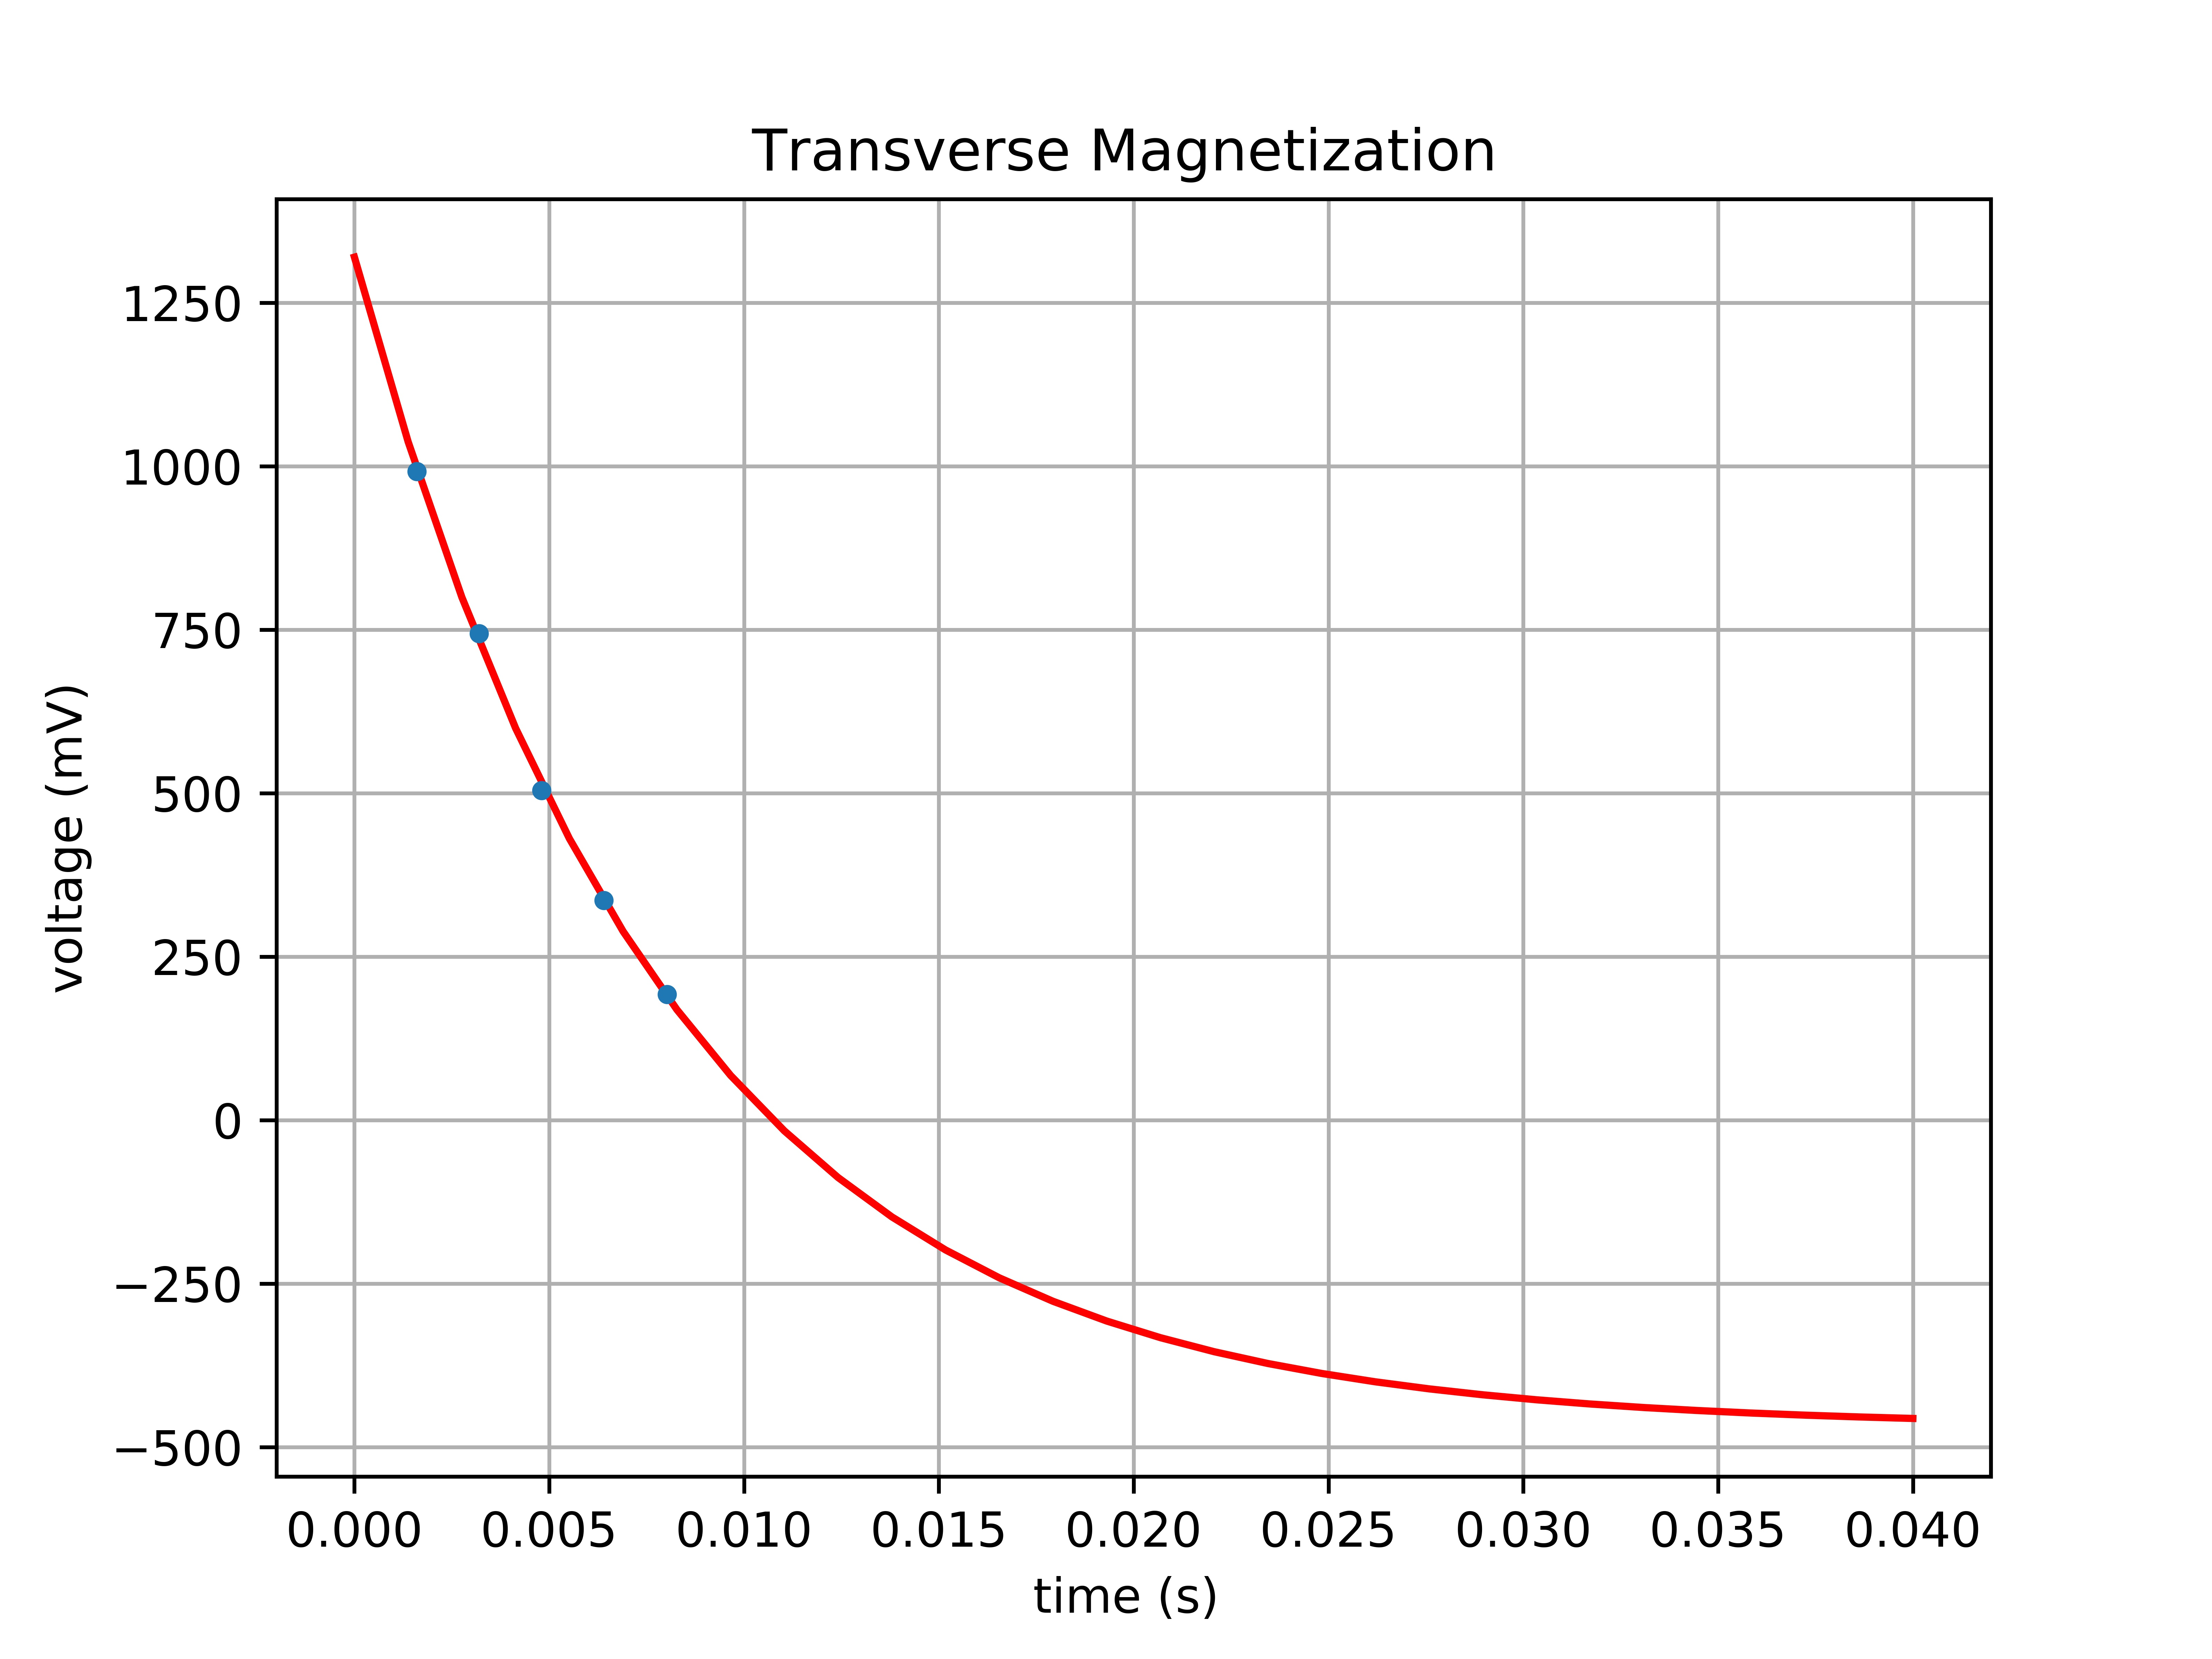
\includegraphics[width=8cm]{Carr} 

\caption{The decay observed for the Carr-Purchell Method of finding $T_{2}$. Vertical error bars are 0.18 mV, measured by amplitude fluctuations.}
\end{figure}

\subsubsection{Meiboom-Gill multiple pulse method}

\begin{figure}[h]

\centering
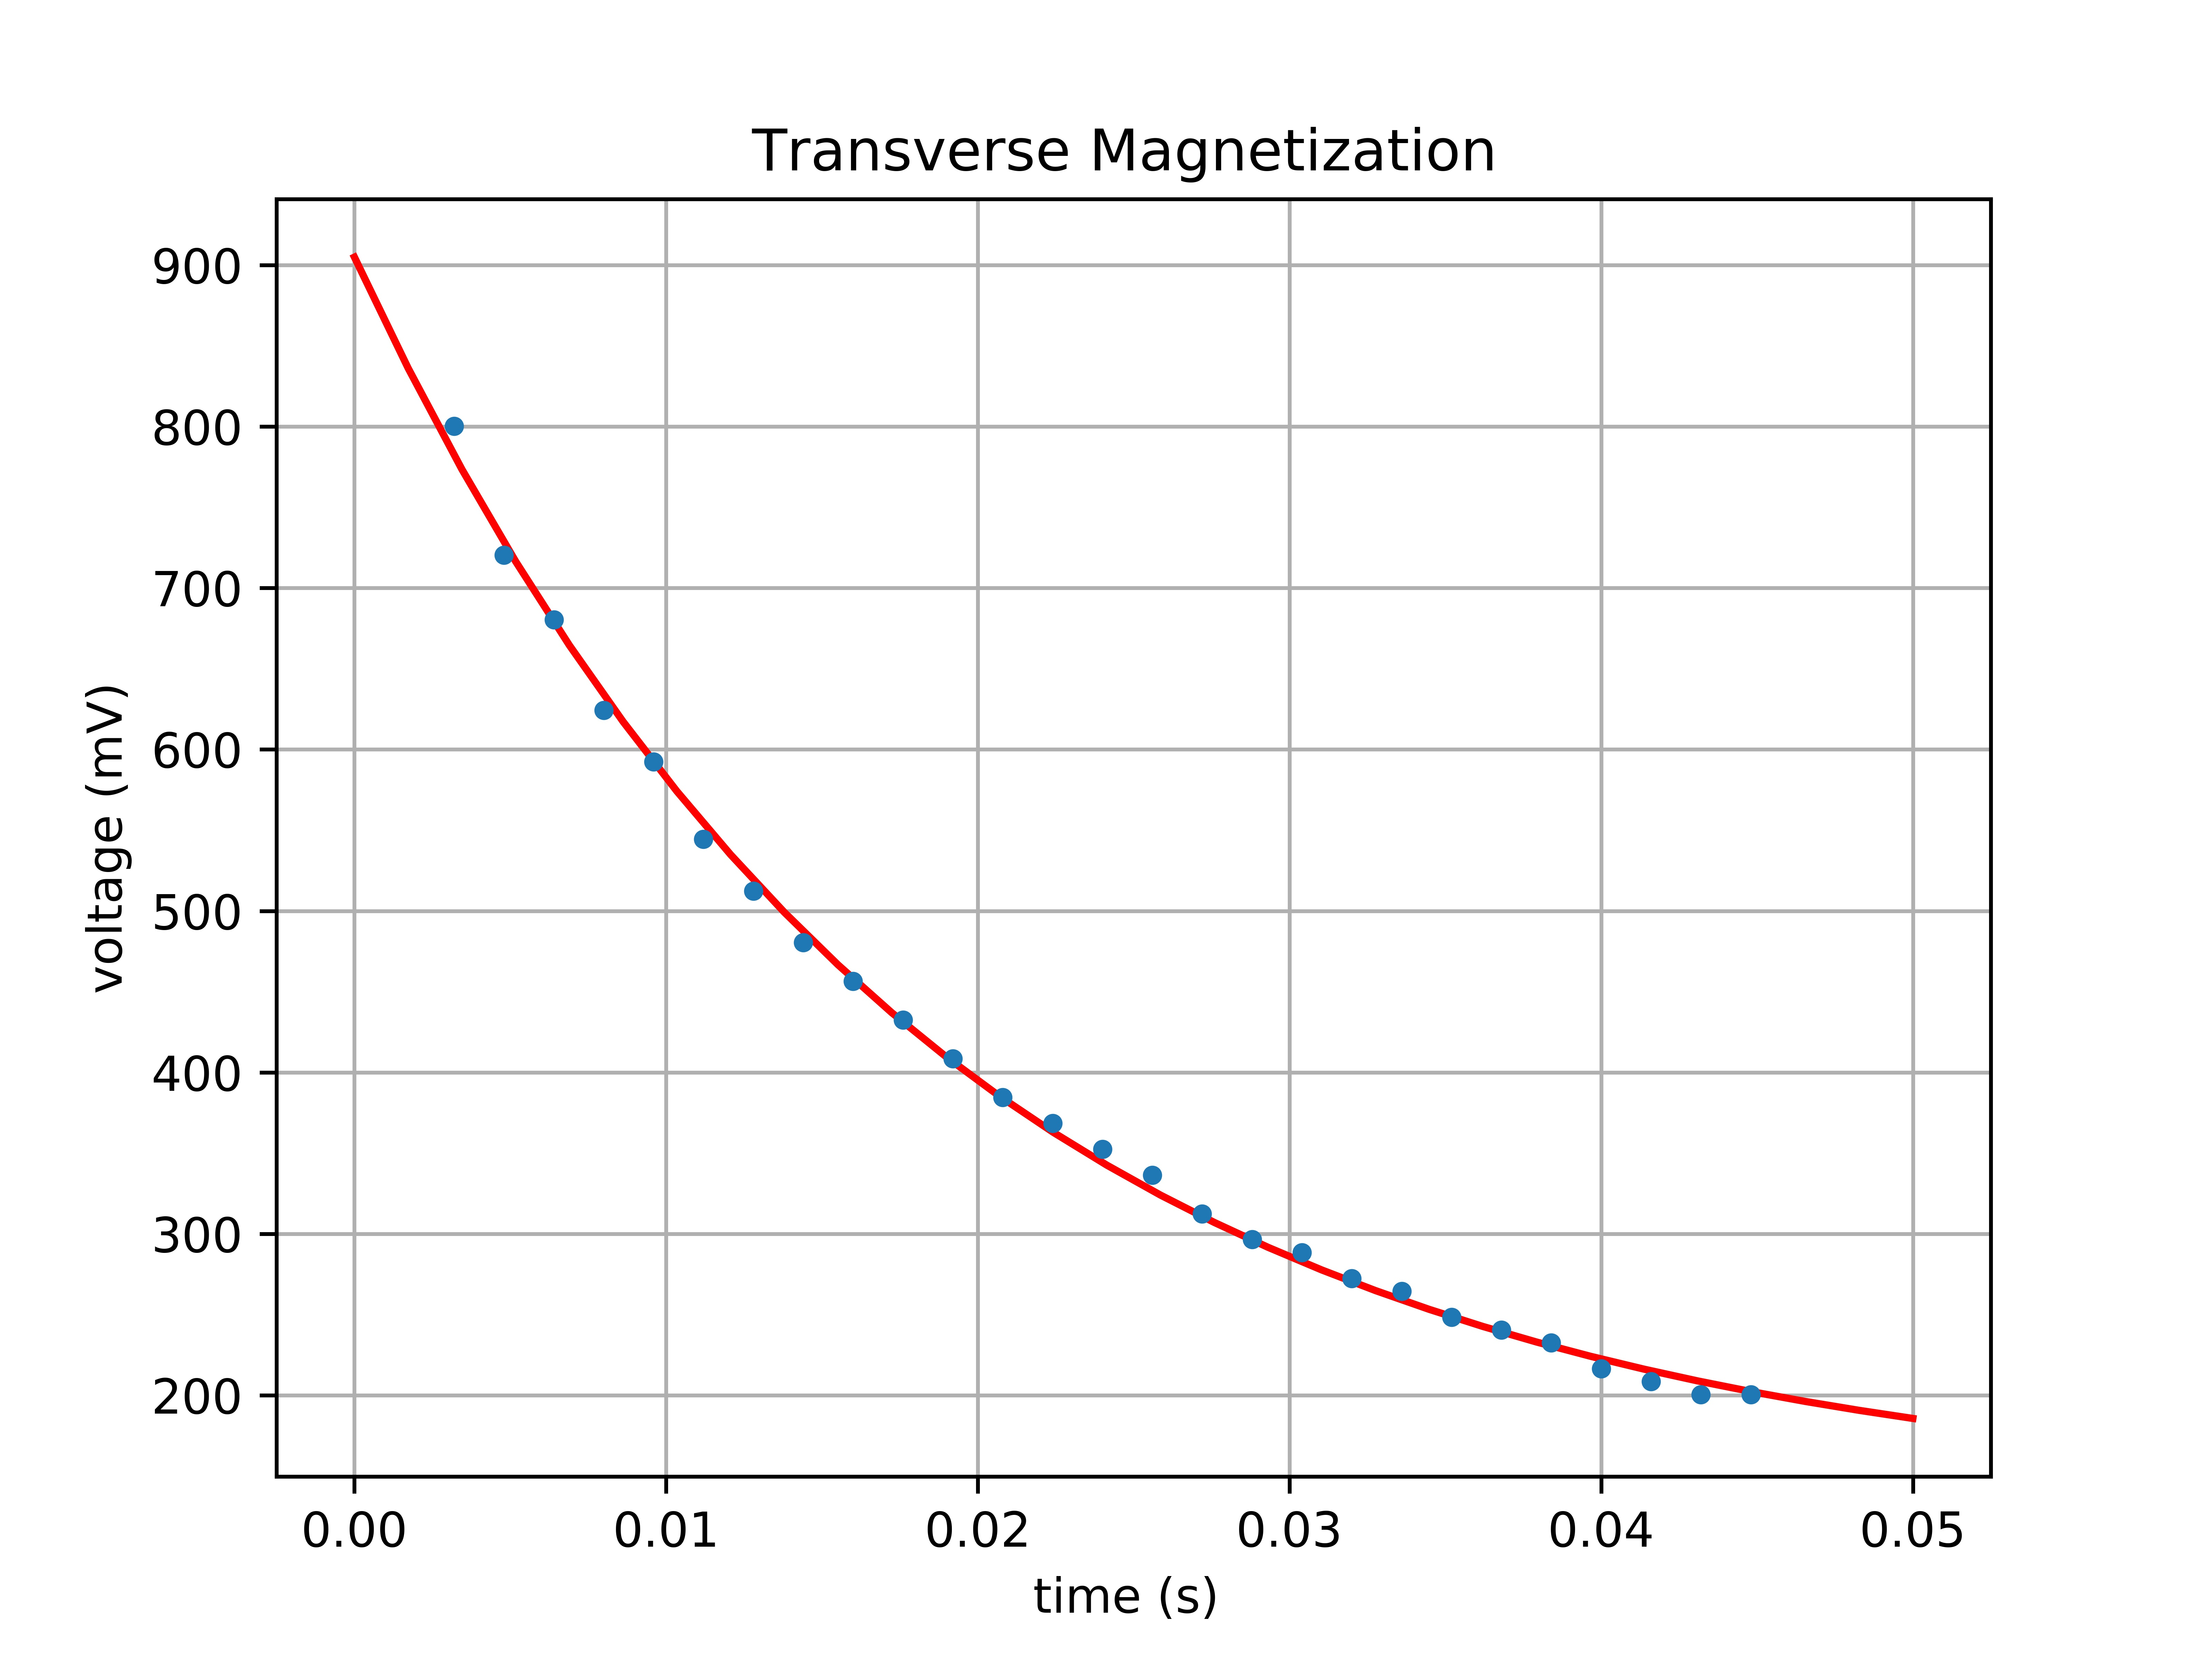
\includegraphics[width=8cm]{Mei} 

\caption{The decay observed for the Meiboom-Gill Method of finding $T_{2}$. Vertical error bars are 0.022 mV from amplitude flucuations.}
\end{figure}

As can be seen, the Meiboom-Gill method results in a decay longer than the Carr-Purchell decay, and is more accurate for error compounding reasons discussed in section $0.1.4$. The decay is depicted in (Fig. 6) and is found to be $T_{2} = 18.4409 \pm 0.34106 $ ms, with the uncertainty found using a bump up/down method.


\section{Error Analysis}

The $T_{1}$ measurement had a wide uncertainty due to there being a lack of data measurements around the zero-crossing time $t_{0}$.
For $T_{2}$, the data taken resembled not a bell-shaped distribution, but an increasing distribution as the delay time increased. Assuming that there would ideally be a bell-shaped distribution if more data was taken with longer delay times, this would mean that the center, or the actual value of $T_{2}$ is most precise with our longest delay time measurement, but might be a higher value. The problem which occurs with increasing the delay time is that measured points become indistinguishable from each other when approaching the end of a decaying exponential. Therefore, a lot of the fit relies on the early points. This questions to the validity of how our exponential fit was applied, and perhaps a different method of fitting should be looked into.
Random errors as found by the amplitude fluctuations proved to be minuscule using the bump up and down method. 
All of the data included some sort of vertical threshold noise. However, since the data dealt with the time domain, this was negligible.
The effect of a resonant frequency uncertainty should be looked more into, perhaps by measuring the time decay deviations when the resonant frequency is fluctuated.
Interesting to note is that the Carr-Purchell method yielded a smaller $T_{2}$ than the Hahn method. This is perhaps an indicator that the Carr-Purchell degree error does in fact compound quickly. 
Because the data taken assumed a primarily homogenous field and a centered sample, these should be looked into by minimizing the field gradient and by seeing how the sample's position affects recorded values. Because the field homogeneity is complicated to adjust, one solution to somewhat minimizing its effects would be to lower the thermal temperature of where it is placed.
A fine-adjuster for the sample's position within the magnet would be useful for centering and seeing the resulting effects. Such an adjuster can perhaps be implemented in future experiments.
	
	
\section{Conclusions}

Mineral oil was situated in a NMR spectrometer and magnet apparatus. A resonant frequency for the sample was found by minimizing the beat frequency. 90 and 180 degree pulses were calibrated by seeing their effect on the magnet's output signal. Following, an approximation of $\Delta B_{0}$ was obtained by observing the decay after a 90 degree pulse. Next, $T_{1}$ was calculated using the decay of a 180 to 90 pulse. Different values for $T_{2}$ were then found using the Hahn two pulse method and the multiple pulse methods of Carr-Purchell and Meiboom-Gill. The multiple pulse methods saw an increasing relationship with delay time and $T_{2}$. To improve results, more data measurements for the $T_{1}$ measurement could be taken around the zero crossing time and a longer interval could have been used for the $T_{2}$ methods. Overall, random noise had small effects and the effects of having a resonant frequency deviation should be looked into. 


\section{Acknowledgements}

Acknowledgements to Joe Schindler for assistance with operating the apparatus.

\section{References}

	Melissinos and Napolitano, Experiments in Modern Physics, 2nd Edition, pp 252-273. Academic Press, 2003.

\smallskip

	University of California, Santa Cruz Physics 134 Advanced Physics Laboratory Winter 2019 Lab Manual

\smallskip

	Wolff-Reichert, Pulsed Magnetic Resonance Spectrometer, Teach-Spin, Inc., 1997.




%\begin{figure}[h]

%\centering
%\includegraphics[width=10cm]{polarizer} 

%\caption{Values of  $\frac{\Delta E}{\mu_{0} B}$, the distance between the lines split from a magnetic field to the initial line of zero magnetic field.}

%\end{figure}



\end{document}